% direction4.tex
% Build: pdflatex direction4.tex
% A standalone one-page reproduction of "Card 4" — Direction 4:
% Palette of ansätze (top band) + Pipeline with bifurcation (bottom band).
%
% Self-contained — only requires a standard pdflatex install with TikZ.

\documentclass[tikz,border=8pt]{standalone}

\usepackage[utf8]{inputenc}
\usepackage[T1]{fontenc}
\usepackage{lmodern}
\usepackage{amsmath,amssymb}
\usepackage{xcolor}
\usepackage{tikz}
\usetikzlibrary{positioning,calc,arrows.meta,shapes.geometric,backgrounds,fit}

% ---------- palette (matches direction4-palette.jsx) ----------
\definecolor{bgcol}{HTML}{faf8f4}
\definecolor{ink}{HTML}{1a1d24}
\definecolor{faint}{HTML}{6b6f78}
\definecolor{rulecol}{HTML}{d8d4cc}
\definecolor{hairline}{HTML}{e4e0d7}
\definecolor{accent}{HTML}{3d5a9e}
\definecolor{amber}{HTML}{b8892e}
\definecolor{paper}{HTML}{ffffff}
\definecolor{ringBg}{HTML}{eaedf5}
\definecolor{ringBorder}{HTML}{9aa4c0}
\definecolor{odeBg}{HTML}{f6e7cf}
\definecolor{odeBorder}{HTML}{c99b5a}
\definecolor{algBg}{HTML}{e5ecd9}
\definecolor{algBorder}{HTML}{8faa70}

% ---------- styling helpers ----------
\newcommand{\stagehead}[2]{%
  {\ttfamily\scriptsize\color{faint}0#1}\hspace{0.4em}%
  {\bfseries\small\color{ink}#2}%
}
\newcommand{\upper}[1]{{\ttfamily\fontsize{6.2pt}{7.5pt}\selectfont\MakeUppercase{#1}}}

% ---------- TikZ styles ----------
\tikzset{
  every node/.style={inner sep=0pt, outer sep=0pt},
  card/.style={draw=rulecol, fill=paper, line width=0.3pt},
  cardA/.style={draw=accent, fill=paper, line width=0.6pt},
  cardAmber/.style={draw=amber, fill=paper, line width=0.6pt},
  mini/.style={draw=rulecol, fill=paper, line width=0.3pt,
               minimum width=33mm, minimum height=23mm},
  miniSel/.style={draw=accent, fill=paper, line width=0.5pt,
                  minimum width=33mm, minimum height=23mm},
  arrowhead/.style={-{Stealth[length=1.6mm,width=1.4mm]}, line width=0.35pt, color=faint},
  faintrule/.style={draw=rulecol, line width=0.25pt},
  hairrule/.style={draw=hairline, line width=0.2pt},
}

\begin{document}

% Overall artboard: 1328 x 531 px.  We scale to mm using 1 mm = ~5.64 px,
% giving an artboard ≈ 235 mm x 94 mm.  Standalone crops to content + border.
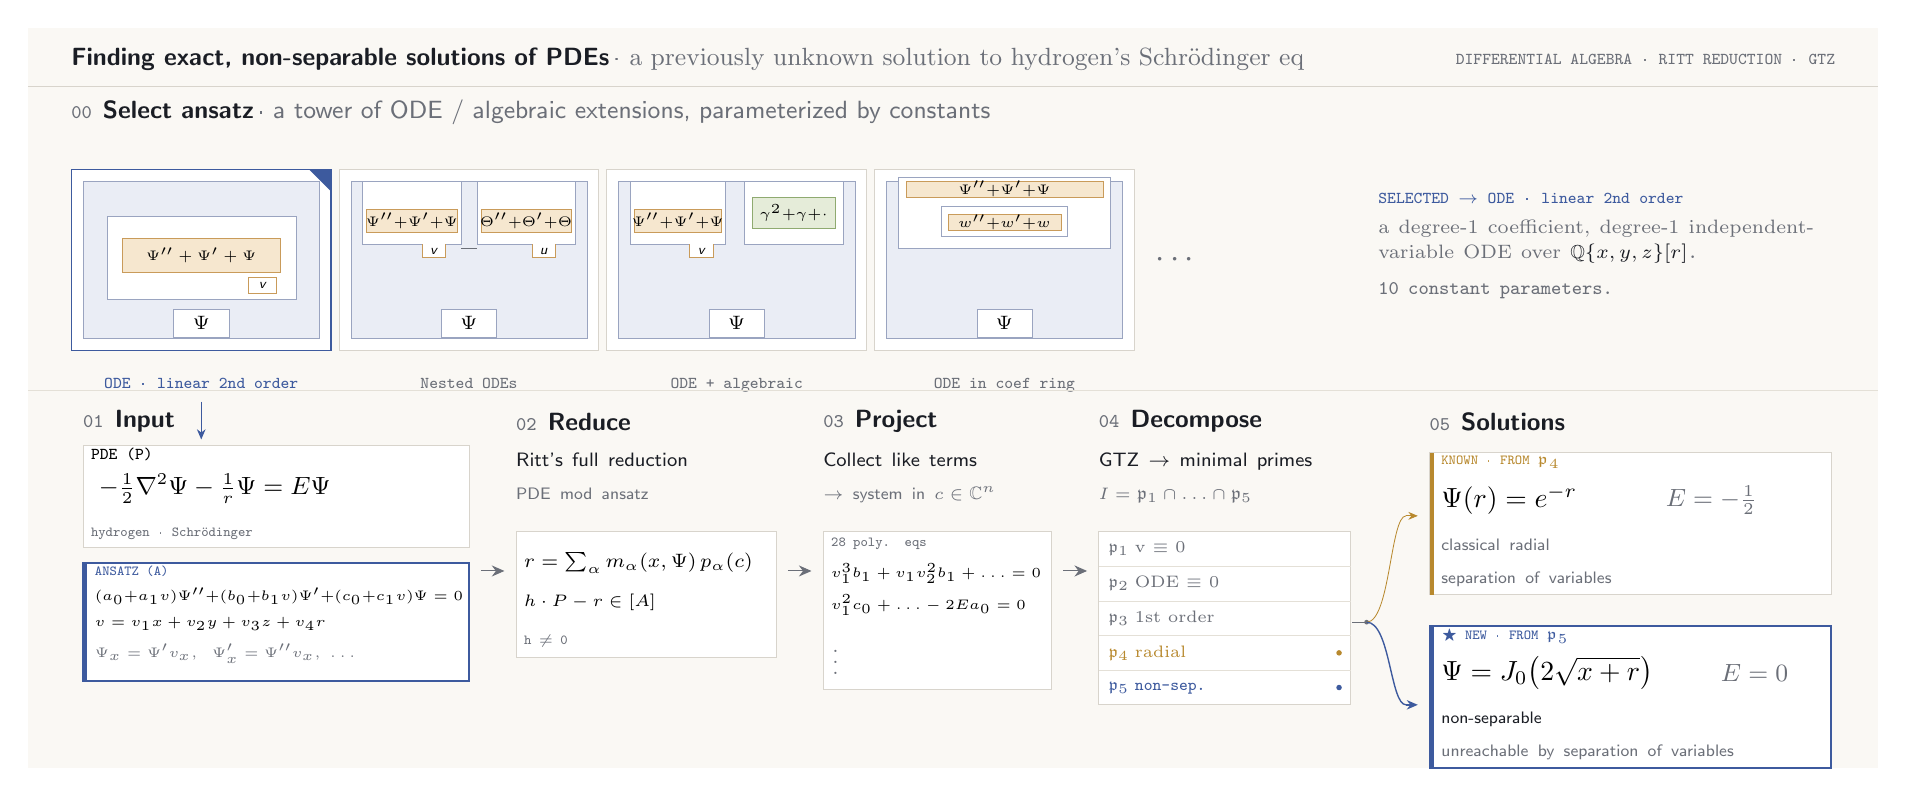
\begin{tikzpicture}[x=1mm, y=1mm, font=\sffamily]

% ========== BACKGROUND ==========
\fill[bgcol] (0,0) rectangle (235, 94);

% ========== HEADER STRIP ==========
\node[anchor=west] at (5.5, 90)
  {\bfseries\small\color{ink} Finding exact, non-separable solutions of PDEs%
   \color{faint}\normalfont\,\textperiodcentered\ a previously unknown solution to hydrogen's Schr\"odinger eq};
\node[anchor=east] at (229.5, 90)
  {\ttfamily\color{faint}\fontsize{6.5pt}{7.8pt}\selectfont
   DIFFERENTIAL ALGEBRA \textperiodcentered\ RITT REDUCTION \textperiodcentered\ GTZ};
\draw[faintrule] (0, 86.5) -- (235, 86.5);

% ========== TOP BAND — ANSATZ PALETTE ==========
\node[anchor=west] at (5.5, 83.2)
  {\stagehead{0}{Select ansatz}\,%
   \color{faint}\small\textperiodcentered\ a tower of ODE / algebraic extensions, parameterized by constants};

% ----- mini ansatz frames (24mm tall + label) -----
% Positioned left-to-right; y baseline for box top at ~76, bottom at ~53
\def\miniY{64.5}          % y-center of mini card
\def\miniLblY{49.5}       % y of the caption

% ---- A · single ODE (selected) ----
\begin{scope}[shift={(22, \miniY)}]
  \node[miniSel] (mA) at (0,0) {};
  % ring background
  \fill[ringBg, draw=ringBorder, line width=0.15pt]
       ($(mA.south west)+(1.5,1.5)$) rectangle ($(mA.north east)+(-1.5,-1.5)$);
  % inner ring paper
  \fill[paper, draw=ringBorder, line width=0.15pt]
       (-12, -5) rectangle (12, 5.5);
  % ODE strip
  \fill[odeBg, draw=odeBorder, line width=0.15pt]
       (-10, -1.6) rectangle (10, 2.8);
  \node at (0, 0.6) {\fontsize{5.5pt}{6.5pt}\selectfont\itshape $\Psi''+\Psi'+\Psi$};
  % v box
  \draw[odeBorder, line width=0.15pt, fill=paper]
       (6, -4.2) rectangle (9.5, -2.2);
  \node at (7.75, -3.2) {\fontsize{5pt}{6pt}\selectfont\itshape v};
  % Psi output
  \draw[ringBorder, line width=0.2pt, fill=paper]
       (-3.5, -9.8) rectangle (3.5, -6.3);
  \node at (0, -8.05) {\fontsize{7pt}{8pt}\selectfont\itshape$\Psi$};
  % selected corner fold
  \fill[accent] ($(mA.north east)+(-2.8,0)$) -- ($(mA.north east)$) --
                ($(mA.north east)+(0,-2.8)$) -- cycle;
\end{scope}
\node[anchor=north] at (22, \miniLblY)
  {\ttfamily\fontsize{6pt}{7.2pt}\selectfont\color{accent}\bfseries ODE \textperiodcentered\ linear 2nd order};

% ---- B · nested ODEs ----
\begin{scope}[shift={(56, \miniY)}]
  \node[mini] (mB) at (0,0) {};
  \fill[ringBg, draw=ringBorder, line width=0.15pt]
       ($(mB.south west)+(1.5,1.5)$) rectangle ($(mB.north east)+(-1.5,-1.5)$);
  % outer ODE
  \fill[paper, draw=ringBorder, line width=0.15pt] (-13.5,2) rectangle (-1,10);
  \fill[odeBg, draw=odeBorder, line width=0.15pt] (-13,3.5) rectangle (-1.5,6.5);
  \node at (-7.25, 5)  {\fontsize{4.5pt}{5.5pt}\selectfont\itshape $\Psi''{+}\Psi'{+}\Psi$};
  \draw[odeBorder, line width=0.15pt, fill=paper] (-6,2) -- (-6,0.3) -- (-3,0.3) -- (-3,2);
  \node at (-4.5, 1.1) {\fontsize{4.5pt}{5.5pt}\selectfont\itshape v};
  % inner ODE
  \fill[paper, draw=ringBorder, line width=0.15pt] (1,2) rectangle (13.5,10);
  \fill[odeBg, draw=odeBorder, line width=0.15pt] (1.5,3.5) rectangle (13,6.5);
  \node at (7.25, 5)   {\fontsize{4.5pt}{5.5pt}\selectfont\itshape $\Theta''{+}\Theta'{+}\Theta$};
  \draw[odeBorder, line width=0.15pt, fill=paper] (8,2) -- (8,0.3) -- (11,0.3) -- (11,2);
  \node at (9.5, 1.1) {\fontsize{4.5pt}{5.5pt}\selectfont\itshape u};
  % connector between them
  \draw[faint, line width=0.15pt] (-1,1.5) -- (1,1.5);
  % Psi output
  \draw[ringBorder, line width=0.2pt, fill=paper]
       (-3.5, -9.8) rectangle (3.5, -6.3);
  \node at (0, -8.05) {\fontsize{7pt}{8pt}\selectfont\itshape$\Psi$};
\end{scope}
\node[anchor=north] at (56, \miniLblY)
  {\ttfamily\fontsize{6pt}{7.2pt}\selectfont\color{faint} Nested ODEs};

% ---- C · ODE + algebraic ----
\begin{scope}[shift={(90, \miniY)}]
  \node[mini] (mC) at (0,0) {};
  \fill[ringBg, draw=ringBorder, line width=0.15pt]
       ($(mC.south west)+(1.5,1.5)$) rectangle ($(mC.north east)+(-1.5,-1.5)$);
  % ODE
  \fill[paper, draw=ringBorder, line width=0.15pt] (-13.5,2) rectangle (-1.5,10);
  \fill[odeBg, draw=odeBorder, line width=0.15pt] (-13,3.5) rectangle (-2,6.5);
  \node at (-7.5, 5)  {\fontsize{4.5pt}{5.5pt}\selectfont\itshape $\Psi''{+}\Psi'{+}\Psi$};
  \draw[odeBorder, line width=0.15pt, fill=paper] (-6,2) -- (-6,0.3) -- (-3,0.3) -- (-3,2);
  \node at (-4.5, 1.1) {\fontsize{4.5pt}{5.5pt}\selectfont\itshape v};
  % algebraic ext (green)
  \fill[paper, draw=ringBorder, line width=0.15pt] (1,2) rectangle (13.5,10);
  \fill[algBg, draw=algBorder, line width=0.15pt] (2,4) rectangle (12.5,8);
  \node at (7.25, 6) {\fontsize{5pt}{6pt}\selectfont\itshape $\gamma^2{+}\gamma{+}\cdot$};
  % Psi output
  \draw[ringBorder, line width=0.2pt, fill=paper]
       (-3.5, -9.8) rectangle (3.5, -6.3);
  \node at (0, -8.05) {\fontsize{7pt}{8pt}\selectfont\itshape$\Psi$};
\end{scope}
\node[anchor=north] at (90, \miniLblY)
  {\ttfamily\fontsize{6pt}{7.2pt}\selectfont\color{faint} ODE + algebraic};

% ---- D · ODE in coef ring ----
\begin{scope}[shift={(124, \miniY)}]
  \node[mini] (mD) at (0,0) {};
  \fill[ringBg, draw=ringBorder, line width=0.15pt]
       ($(mD.south west)+(1.5,1.5)$) rectangle ($(mD.north east)+(-1.5,-1.5)$);
  % outer ODE
  \fill[paper, draw=ringBorder, line width=0.15pt] (-13.5,1.5) rectangle (13.5,10.5);
  \fill[odeBg, draw=odeBorder, line width=0.15pt] (-12.5,8) rectangle (12.5,10);
  \node at (0, 9) {\fontsize{4.5pt}{5.5pt}\selectfont\itshape $\Psi''{+}\Psi'{+}\Psi$};
  % nested w ODE
  \fill[paper, draw=ringBorder, line width=0.15pt] (-8,3) rectangle (8,6.8);
  \fill[odeBg, draw=odeBorder, line width=0.15pt] (-7.2,3.8) rectangle (7.2,5.8);
  \node at (0, 4.8) {\fontsize{4pt}{5pt}\selectfont\itshape $w''{+}w'{+}w$};
  % Psi output
  \draw[ringBorder, line width=0.2pt, fill=paper]
       (-3.5, -9.8) rectangle (3.5, -6.3);
  \node at (0, -8.05) {\fontsize{7pt}{8pt}\selectfont\itshape$\Psi$};
\end{scope}
\node[anchor=north] at (124, \miniLblY)
  {\ttfamily\fontsize{6pt}{7.2pt}\selectfont\color{faint} ODE in coef ring};

% ---- ellipsis ----
\node at (146, \miniY) {\ttfamily\color{faint}\large$\cdots$};

% ---- right-aligned selected caption ----
\node[anchor=north east, text width=58mm, align=left] at (229.5, 73) {%
  \ttfamily\fontsize{6.5pt}{9pt}\selectfont\color{accent}\bfseries SELECTED $\rightarrow$ ODE \textperiodcentered\ linear 2nd order\\[2pt]%
  \normalfont\color{faint}\fontsize{6.8pt}{9pt}\selectfont
  a degree-1 coefficient, degree-1 independent-variable ODE over
  \color{ink}\ttfamily$\mathbb{Q}\{x,y,z\}[r]$\color{faint}.\\[1pt]
  10 constant parameters.
};

% hairline under palette band
\draw[hairrule] (0, 48) -- (235, 48);

% dropper line down from selected ansatz into pipeline (lowered to clear caption)
\draw[accent, line width=0.4pt] (22, 46.5) -- (22, 43);
\draw[accent, line width=0.4pt, -{Stealth[length=1.3mm,width=1.1mm]}]
      (22, 43) -- (22, 41.7);

% ========== BOTTOM BAND — PIPELINE ==========
% Five stages: Input, Reduce, Project, Decompose, Solutions, with arrows.
% x layout (left→right):
%  01 Input   : 7  .. 46
%  →
%  02 Reduce  : 52 .. 80
%  →
%  03 Project : 86 .. 114
%  →
%  04 Decomp  : 120 .. 154
%  bifurcation : 154 .. 165
%  05 Sol     : 166 .. 229

% ---------- 01 INPUT ----------
\node[anchor=west] at (7, 44)  {\stagehead{1}{Input}};
% PDE card
\draw[card] (7, 28) rectangle (56, 41);
\node[anchor=north west] at (8, 40.6) {\upper{PDE\ (P)}};
\node[anchor=west] at (9, 35.5)
  {\small$-\tfrac{1}{2}\nabla^{2}\Psi - \tfrac{1}{r}\Psi = E\Psi$};
\node[anchor=south west] at (8, 29)
  {\ttfamily\fontsize{5.5pt}{6.5pt}\selectfont\color{faint} hydrogen \textperiodcentered\ Schr\"odinger};
% Ansatz card
\draw[cardA] (7, 11) rectangle (56, 26);
\draw[accent, line width=1.2pt] (7.3, 11) -- (7.3, 26); % left accent bar
\node[anchor=north west] at (8.5, 25.6)
  {\ttfamily\fontsize{5.5pt}{6.5pt}\selectfont\color{accent}\bfseries ANSATZ\ (A)};
\node[anchor=west] at (8.5, 21.8)
  {\fontsize{5.2pt}{6pt}\selectfont$(a_0{+}a_1 v)\Psi''{+}(b_0{+}b_1 v)\Psi'{+}(c_0{+}c_1 v)\Psi = 0$};
\node[anchor=west] at (8.5, 18.3)
  {\fontsize{5.5pt}{6.5pt}\selectfont$v = v_1 x + v_2 y + v_3 z + v_4 r$};
\node[anchor=west] at (8.5, 14.5)
  {\fontsize{5pt}{6pt}\selectfont\color{faint}$\Psi_x = \Psi' v_x,\;\; \Psi'_x = \Psi'' v_x,\;\ldots$};

\draw[arrowhead] (57.5, 25) -- (60.5, 25);

% ---------- 02 REDUCE ----------
\node[anchor=west] at (62, 44) {\stagehead{2}{Reduce}};
\node[anchor=north west, text width=30mm] at (62, 40)
  {\fontsize{7pt}{9pt}\selectfont\color{ink} Ritt's full reduction\\
   \color{faint}\fontsize{6.5pt}{8pt}\selectfont PDE mod ansatz};
\draw[card] (62, 14) rectangle (95, 30);
\node[anchor=west] at (63, 26)
  {\fontsize{7pt}{8pt}\selectfont$r = \sum_\alpha m_\alpha(x,\Psi)\, p_\alpha(c)$};
\node[anchor=west] at (63, 21)
  {\fontsize{6.5pt}{7.5pt}\selectfont$h \cdot P - r \in [A]$};
\node[anchor=south west] at (63, 15.3)
  {\ttfamily\fontsize{5.5pt}{6.5pt}\selectfont\color{faint} h $\neq$ 0};

\draw[arrowhead] (96.5, 25) -- (99.5, 25);

% ---------- 03 PROJECT ----------
\node[anchor=west] at (101, 44) {\stagehead{3}{Project}};
\node[anchor=north west, text width=30mm] at (101, 40)
  {\fontsize{7pt}{9pt}\selectfont\color{ink} Collect like terms\\
   \color{faint}\fontsize{6.5pt}{8pt}\selectfont $\rightarrow$ system in $c \in \mathbb{C}^n$};
\draw[card] (101, 10) rectangle (130, 30);
\node[anchor=north west] at (102, 29.2)
  {\ttfamily\fontsize{5.5pt}{6.5pt}\selectfont\color{faint} 28 poly. eqs};
\node[anchor=north west] at (102, 26)
  {\ttfamily\fontsize{5.5pt}{7pt}\selectfont $v_1^3 b_1 + v_1 v_2^2 b_1 + \ldots = 0$};
\node[anchor=north west] at (102, 22)
  {\ttfamily\fontsize{5.5pt}{7pt}\selectfont $v_1^2 c_0 + \ldots - 2 E a_0 = 0$};
\node[anchor=north west] at (102, 17)
  {\ttfamily\fontsize{6pt}{7pt}\selectfont\color{faint} $\vdots$};

\draw[arrowhead] (131.5, 25) -- (134.5, 25);

% ---------- 04 DECOMPOSE ----------
\node[anchor=west] at (136, 44) {\stagehead{4}{Decompose}};
\node[anchor=north west, text width=32mm] at (136, 40)
  {\fontsize{7pt}{9pt}\selectfont\color{ink} GTZ $\rightarrow$ minimal primes\\
   \color{faint}\fontsize{6.5pt}{8pt}\selectfont $I = \mathfrak{p}_1 \cap \ldots \cap \mathfrak{p}_5$};
% table of primes
\draw[card] (136, 8) rectangle (168, 30);
\foreach \i in {1,2,3,4} {
  \draw[hairrule] (136, 30 - \i*4.4) -- (168, 30 - \i*4.4);
}
\node[anchor=west] at (137.2, 27.8)
  {\ttfamily\fontsize{6pt}{7pt}\selectfont\color{faint}\bfseries $\mathfrak{p}_1$\,\,\normalfont v $\equiv$ 0};
\node[anchor=west] at (137.2, 23.4)
  {\ttfamily\fontsize{6pt}{7pt}\selectfont\color{faint}\bfseries $\mathfrak{p}_2$\,\,\normalfont ODE $\equiv$ 0};
\node[anchor=west] at (137.2, 19.0)
  {\ttfamily\fontsize{6pt}{7pt}\selectfont\color{faint}\bfseries $\mathfrak{p}_3$\,\,\normalfont 1st order};
\node[anchor=west] at (137.2, 14.6)
  {\ttfamily\fontsize{6pt}{7pt}\selectfont\color{amber}\bfseries $\mathfrak{p}_4$\,\,\normalfont radial};
\fill[amber] (166.5, 14.6) circle (0.35);
\node[anchor=west] at (137.2, 10.2)
  {\ttfamily\fontsize{6pt}{7pt}\selectfont\color{accent}\bfseries $\mathfrak{p}_5$\,\,non-sep.};
\fill[accent] (166.5, 10.2) circle (0.35);

% ---------- BIFURCATION CONNECTOR ----------
\draw[faint, line width=0.25pt] (168.2, 18.5) -- (170, 18.5);
\fill[faint] (170, 18.5) circle (0.3);
\draw[amber, line width=0.3pt]
  (170, 18.5) .. controls (173, 18.5) and (173, 32) .. (175, 32);
\draw[amber, line width=0.3pt, -{Stealth[length=1.2mm,width=1mm]}]
  (175, 32) -- (176.5, 32);
\draw[accent, line width=0.5pt]
  (170, 18.5) .. controls (173, 18.5) and (173, 8) .. (175, 8);
\draw[accent, line width=0.5pt, -{Stealth[length=1.4mm,width=1.2mm]}]
  (175, 8) -- (176.5, 8);

% ---------- 05 SOLUTIONS ----------
\node[anchor=west] at (178, 44) {\stagehead{5}{Solutions}};

% Known (amber)
\draw[card] (178, 22) rectangle (229, 40);
\draw[amber, line width=1.2pt] (178.3, 22) -- (178.3, 40);
\node[anchor=north west] at (179.5, 39.6)
  {\ttfamily\fontsize{5.5pt}{6.5pt}\selectfont\color{amber}\bfseries KNOWN \textperiodcentered\ FROM $\mathfrak{p}_4$};
\node[anchor=west] at (179.5, 34) {\normalsize$\Psi(r) = e^{-r}$};
\node[anchor=west] at (208, 34) {\small\color{faint}$E = -\tfrac{1}{2}$};
\node[anchor=south west, text width=50mm, align=left] at (179.5, 23)
  {\fontsize{6pt}{7.5pt}\selectfont\color{faint}classical radial\\
   separation of variables};

% New (accent)
\draw[cardA] (178, 0) rectangle (229, 18);
\draw[accent, line width=1.2pt] (178.3, 0) -- (178.3, 18);
\node[anchor=north west] at (179.5, 17.6)
  {\ttfamily\fontsize{5.5pt}{6.5pt}\selectfont\color{accent}\bfseries $\bigstar$\ NEW \textperiodcentered\ FROM $\mathfrak{p}_5$};
\node[anchor=west] at (179.5, 12)
  {\normalsize$\Psi = J_0\!\left(2\sqrt{x+r}\right)$};
\node[anchor=west] at (215, 12) {\small\color{faint}$E = 0$};
\node[anchor=south west, text width=50mm, align=left] at (179.5, 1)
  {\fontsize{6pt}{7.5pt}\selectfont\color{ink}non-separable\\
   \color{faint}unreachable by separation of variables};

\end{tikzpicture}
\end{document}
